% !TeX TS-program = Lualatex
% !TeX encoding = UTF-8 Unicode
% !TeX spellcheck = en
% !BIB TS-program = bibtex
% -*- coding: UTF-8; -*-
% vim: set fenc=utf-8
%%%%%%%%%%%%%%%%%%%%%%%%%%%%%%%%%%%%%%%%%%%%%%%%%%%%%%%%%%%%%%%%%%%%%
% 
\documentclass[runningheads]{llncs}
%
\usepackage[T1]{fontenc}
%
% \usepackage[utf8]{inputenc}
% \usepackage{times}
% \usepackage{wrapfig}
\usepackage{graphicx}
% \usepackage{floatrow}
% \usepackage{multicol}
\usepackage{amssymb}
\usepackage{amsmath}
\usepackage{hyperref}
\usepackage{siunitx}
\sisetup{output-exponent-marker=\ensuremath{\mathrm{e}}}
%%%%%%%%%%%%%%%%%%%%%%%%%%%%%%%%%%%%%%%%%%%%%%%%%%%%%%%%%%%%%%%%%%%%%
% NOTATIONS
% Pixel world 
\newcommand{\presynaddr}{a} % pre address
\newcommand{\postsynaddr}{b} % post address
\newcommand{\numevent}{N_{ev}} % total number of events
\newcommand{\presynaddrspace}{\mathcal{A}} %presynaptic address space
\newcommand{\postsynaddrspace}{\mathcal{B}} %postsynaptic address space
\newcommand{\Npol}{N_\text{p}} % number of polarity
\newcommand{\Nneuron}{N_\text{n}} % number of output neurons in the layer
\newcommand{\arank}{r} % address index
\newcommand{\bias}{b} % bias for the MLR model
\newcommand{\synapse}{\mathcal{S}} % synapse
\newcommand{\synapticweight}{w} % synaptic weight
\newcommand{\synapticdelay}{\delta} % synaptic delay
\newcommand{\ranksyn}{s} % synapse index
\newcommand{\Nsyn}{N_{s}} % total number of synapses
\newcommand{\activeweights}{\mathcal{W}} 
\newcommand{\timev}{t} % time
\newcommand{\polev}{p} % polarity
\newcommand{\event}{\epsilon} % event
\newcommand{\eventstream}{\xi} % stream of events
\newcommand{\TS}{S} % time surface
\newcommand{\neuron}{\mathbf{n}} % neuron in the SNN (defined by the spatial position and the channel)
\newcommand{\postneuron}{\mathbf{m}} % post synaptic neuron in the SNN (defined by the spatial position and the kernel)
\newcommand{\channel}{\mathbf{p}} % channel
\newcommand{\layer}{\mathbf{L}} % layer
\newcommand{\ms}{\si{\milli\second}}%
\newcommand{\us}{\si{\micro\second}}%
\newcommand{\timecontext}{T} % time context (cf HOTS) matrice gathering last event times
\newcommand{\current}{I} % post synaptic current
\newcommand{\volt}{u} % membrane potential
\newcommand{\volts}{V} % matrix of membrane potentials
\newcommand{\gain}{\gamma} % homeostatic gain
\newcommand{\simil}{\beta} % similarity value
\newcommand{\Nclass}{N_\text{class}} % number of classes for MLR:
\newcommand{\Nx}{N_\text{X}}
\newcommand{\Ny}{N_\text{Y}}
\newcommand{\Ntime}{N_\text{t}}
\newcommand{\kernel}{K} % convolution kernel
%\newcommand{\kernelind}{\mathbf{k}} % indice of the kernel
\newcommand{\kernelind}{k} % indice of the kernel
\newcommand{\Kx}{K_\text{x}}
\newcommand{\Ky}{K_\text{y}}
\newcommand{\Ktime}{K_\text{t}}
\newcommand{\classiflayer}{\mathbf{C}}
\newcommand{\class}{c} % class k of the MLR
\newcommand{\lrweights}{\theta} % matrix of MLR weights
\newcommand{\lrtrue}{y} % true value of the prediction for MLR
\newcommand{\loss}{J} % cost function for MLR
\newcommand{\softmax}{\sigma}
\newcommand{\actfreq}{f}
\newcommand{\decision}{\hat{y}}
\newcommand{\colorsec}{black}
\newcommand{\colorsubsec}{black}
\newcommand{\speed}{v}
\newcommand{\Nspeed}{N_v}
% Example definitions.
% --------------------
\def\x{{\mathbf x}}
\def\L{{\cal L}}
\newcommand{\fig}[1]{Fig.~\ref{fig:#1}}%{Figure~\ref{fig:#1}}
\DeclareMathOperator*{\argmax}{arg\,max}
\DeclareMathOperator*{\argmin}{arg\,min}

%%%%%%%%%%%%%%%%%%%%%%%%%%%%%%%%%%%%%%%%%%%%%%%%%%%%%%%%%%%%%%%%%%%%%%
% \usepackage{natbib}
% \usepackage[
% %style=chem-acs,
% style=numeric,						% numeric style for reference list
% citestyle=numeric-comp,
% %style=alphabetic-verb,
% giveninits=false,
% maxbibnames=1,
% %firstinits=true,
% %style=apa,
% %maxcitenames=1,
% %maxnames=3,
% %minnames=1,
% %maxbibnames=99,
% dateabbrev=true,
% giveninits=true,
% %uniquename=init,
% url=false,
% doi=false,
% isbn=false,
% eprint=false,
% texencoding=utf8,
% bibencoding=utf8,
% autocite=superscript,boutin_effect_2020
% backend=biber,
% %sorting=none,
% sorting=none,
% sortcites=false,
% %articletitle=false
% ]{biblatex}%

% \bibliography{ref.bib}
%%%%%%%%%%%%%%%%%%%%%%%%%%%%%%%%%%%%%%%%%%%%%%%%%%%%%%%%%%%%%%%%%%%%%%
% \newcommand{\mycaption}[1]{\caption*{#1}}

% \usepackage{titlesec}
% % \titlespacing*{<command>}{<left>}{<before-sep>}{<after-sep>}
% \titlespacing*{\section}
% {0pt}{1.5ex}{0.8ex}
% \titlespacing*{\subsection}
% {0pt}{0.9ex}{0.4ex}
% \titlespacing*{\subsubsection}
% {0pt}{0.5ex}{0.3ex}
% \titlespacing*{\paragraph}{%
%   0pt}{%              left margin
%   0.0\baselineskip}{% space before (vertical)
%   1em}%               space after (horizontal)

% \usepackage{setspace}

\begin{document}

%%%-----------------------------------------------------------------
\title{Accurate detection of spiking motifs in multi-unit raster plots}

\author{
% Miles Keating\orcidID{0009-0000-6871-0373}
% \and
Laurent U Perrinet\orcidID{0000-0002-9536-010X}
\thanks{Funded by A*MIDEX grant AMX-21-RID-025 ``\href{https://laurentperrinet.github.io/grant/polychronies/}{Polychronies}''.}}
%
\authorrunning{LU Perrinet}
% First names are abbreviated in the running head.
% If there are more than two authors, 'et al.' is used.
%
\institute{INT UMR7289, Aix Marseille Univ, CNRS; 27 Bd Moulin, 13005 Marseille, France
% \url{https://laurentperrinet.github.io} \email{laurent.perrinet@univ-amu.fr}
}
%
\maketitle              % typeset the header of the contribution
%
\begin{abstract} 
Recently, there has been a growing interest in exploring the hypothesis that neural activity conveys information through precise spiking motifs. To investigate this phenomenon, various algorithms have been proposed to detect such motifs in Spiking Unit Activity (SUA) recorded from populations of neurons.
In this study, we present a novel detection model that is based on the inversion of a generative model of raster plot synthesis. By leveraging this generative model, we derive an optimal detection procedure, which takes the form of a logistic regression combined with a temporal convolution. One key advantage of this model is its differentiability, allowing us to formulate a supervised learning approach using a gradient descent on the binary cross entropy loss. 
At first, we perform numerical evaluations to assess the model's ability to detect spiking motifs in synthetic data. This analysis highlights the advantages of using spiking motifs over traditional firing-rate-based population codes. Then, we successfully demonstrate that our learning method can recover synthetically generated spiking motifs, indicating its potential for further applications. In the future, we aim to extend this method to real neurobiological data, where the ground truth is unknown, to explore and detect spiking motifs in a more natural and biologically relevant context.
%
\keywords{Neurobiology \and  spike trains \and population coding  \and spiking motifs \and heterogeneous delays \and pattern detection.}
\end{abstract}

%----------------------------%
\section{Introduction}
%---------------------------

%%%%%%%%%%%%%%%%%%%%%%%%%%%%%%%%%%%%%%%%%%%%%
\subsection{The age of large-scale neurobiological event-based data}
%%%%%%%%%%%%%%%%%%%%%%%%%%%%%%%%%%%%%%%%%%%%%
% 
Over the past decade, significant technological advancements in multiple disciplines have expanded the possibilities of studying neuroscience experimentally. These cutting-edge methods integrate various spatial and temporal scales, utilizing techniques such as \textit{in vivo} two-photon imaging, large population recording array technologies, optogenetic circuit control tools, transgenic manipulations, and large volume circuit reconstructions. Leveraging these tools, researchers can now explore neural networks' function, structure, and dynamics with unprecedented precision and detail.

The complexity of the biological reality uncovered by these technologies highlights the importance of neurobiological knowledge in bridging the gap between abstract brain function principles and their biological implementation in neural circuits. Consequently, there is an increasing need to scale up analysis methods to handle the large volumes of data generated by these powerful techniques. Meeting this demand will enable researchers to gain deeper insights into brain function, furthering our understanding of neural circuits and leading to groundbreaking discoveries in neuroscience.

Among the various approaches aimed at addressing this challenge is the Rastermap algorithm~\cite{pachitariu_robustness_2018}. This algorithm effectively rearranges neurons in the raster map based on the similarity of their activity and employs a deconvolution strategy using a linear model. However, it is important to note that the Rastermap algorithm has primarily been tested on calcium imaging data, which may introduce some imprecision in the timing of spiking activity observed in Spiking Unit Activity (SUA) recordings.

Another notable contribution comes from the work of Williams {\it et al.}~\cite{williams_point_2020}. They develop a point process model that addresses limitations in existing models, such as the need for spike times to be discretized or lack of uncertainty estimates for model predictions and estimated parameters. This novel approach characterizes fine-scale sequences at the level of individual spikes and represents sequence occurrences as a few marked events in continuous time. By incorporating learnable time-warping parameters to model sequences of varying durations, the model effectively captures experimentally observed patterns in neural circuits. The authors demonstrate the advantages of their model on experimental recordings from the songbird higher vocal center and the rodent hippocampus.

These advancements in point process modeling and other machine learning-based tools provide valuable opportunities to enhance our understanding of neural circuit function and its underlying mechanisms in complex neural systems.
%
%%%%%%%%%%%%%%%%%%%%%%%%%%%%%%%%%%%%%%%%%%%%%
\subsection{Decoding neural activity using spike distances}
%%%%%%%%%%%%%%%%%%%%%%%%%%%%%%%%%%%%%%%%%%%%%
%
The methods discussed in neuroscience research heavily rely on defining appropriate metrics to compute the distance between spike trains. One well-known measure is the Victor-Purpura distance~\cite{victor_nature_1996}, which effectively addresses inconsistencies observed with firing rate-based estimation of spike trains. Another study refines this metric by incorporating a time constant as a parameter, allowing interpolation between a coincidence detector and a rate difference counter~\cite{van_rossum_novel_2001}. Additionally, these distance measures have been extended to non-Euclidean metrics and morphological manipulations to compute spike train dissimilarity~\cite{kreuz_measuring_2007}. It is suggested that any distance measure could be an optimal solution for a generative model of these measures, possibly through non-linear relations~\cite{aronov_non-euclidean_2004}.

In terms of spike timings, various methods have been developed for estimating the latency of neural responses, including Bayesian binning~\cite{levakova_review_2015}. Unitary event analysis based on a statistical model of chance detection has been widely used to detect significant synchronous patterns above chance in neuron pair recordings~\cite{grun_unitary_2002-1,grun_unitary_2010}. Recent extensions of these methods, such as the 3D-SPADE approach~\cite{stella_3d-spade_2019}, enable the identification of reoccurring patterns in parallel spike train data and assess their statistical significance.

The inclusion of possible temporal dithering in spike timings has been shown to improve performance, particularly in the presence of patterns with varying durations, such as surrogates used to evaluate precisely timed higher order spike correlations~\cite{stella_comparing_2022}. However, some methods may suffer from computational complexity, block-based implementations, and a narrow specialization for specific tasks. To address these challenges, novel methods, like Spikeship~\cite{sotomayor-gomez_spikeship_2021}, have been developed.

The complexity and diversity of these spike train distance and timing comparison methods demonstrate the growing interest in integrating such measures in understanding the neural code. A critical step in testing their potential usefulness is scaling these methods to handle larger amounts of data, enabling broader applications and deeper insights into neural activity patterns and their significance.
%
%%%%%%%%%%%%%%%%%%%%%%%%%%%%%%%%%%%%%%%%%%%%%
\subsection{Detecting spiking motifs with a heterogeneous delays SNN}
%%%%%%%%%%%%%%%%%%%%%%%%%%%%%%%%%%%%%%%%%%%%%
%
These methods highlight the role of spike timing, and a striking example is given for the barn owl auditory system: When it hears the sound of a mouse, this sound generates a specific spiking response in both ears, and in particular, the precise timing between these signals can be used to determine the position of the prey~\cite{goodman_spike-timing-based_2010}. More generally, there is now a large body of literature showing that the dynamics of the brain are often organized into stereotyped sequences (for a review, see~\cite{grimaldi_precise_2023}). 

% We believe that the detection of spiking motifs should be based on a proper understanding of spiking neural networks (SNNs). However, most existing SNNs, especially those adapted from analogous deep learning like architectures, rely on encoding information based on a continuously varying firing rate.
% Notable exceptions of SNNs using precise spike timing are the time coding machine of~\cite{lazar_time_2004} and the 
Here, we propose a new metric inspired by the \textit{polychronization} model of Izhikevich~\cite{izhikevich_polychronization_2006}. This theoretical model is based on a random recurrent model of spiking neurons that includes synaptic delays chosen from a range of biologically realistic delays (from $0$ to $20~\ms$) and whose weights are evolving with a Spike-Time Dependent Plasticity (STDP) learning rule. Delays are defined as the total time taken for a spike to travel from the soma of one presynaptic neuron to that of the efferent postsynaptic neuron. Note that only the weights are changed using the STDP rule, and that the set of delays is randomly set at initialization and then ``frozen'' for the rest of the simulation. 

Due to the interplay between the delays and the STDP, the spiking neurons spontaneously self-organize into groups and %generate patterns of stereotypical polychronous activity, i.e., 
exhibit reproducible time-locked firing patterns, which the author defines as ``polychronous groups''. A key component of this model is the fact that neurons in a polychronous group fire at different times, but thanks to the effect of heterogeneous delays, spikes may converge synchronously on the soma of the postsynaptic neuron: This leads to the summation of the excitatory postsynaptic potentials evoked by each spike, and thus to the crossing of the voltage threshold and the discharge of a spike (see Figure~\ref{fig:izhikevich}). According to the STDP rule, the group of neurons involved in this polychronous activity will see their synaptic weight increase and thus  consolidate the formation of that polychronous group.  A limitation of this model is that these heterogeneous delays are fixed and can not evolve in time.

%----------------------------%
%
\begin{figure}[t]
  \centering
  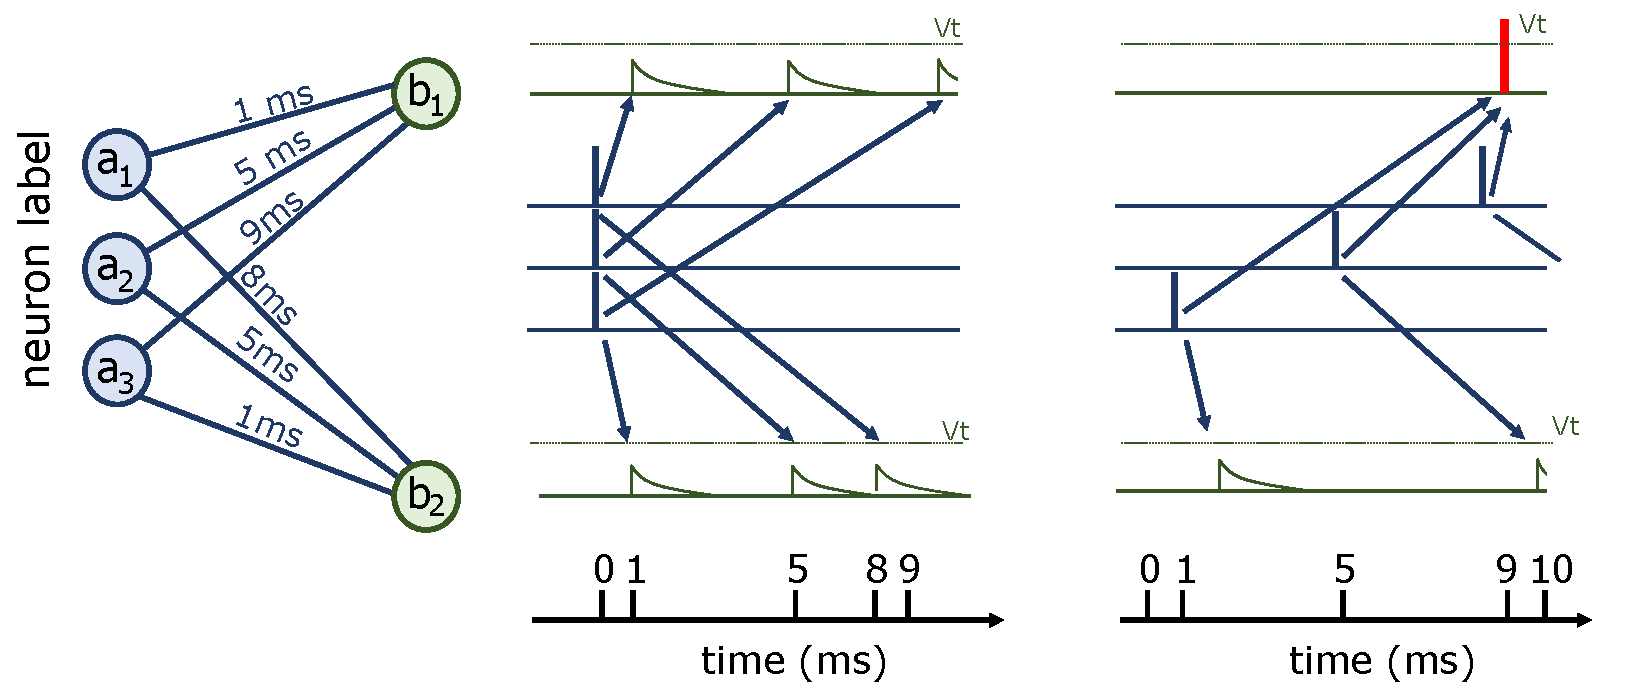
\includegraphics[width=0.95\linewidth]{figures/izhikevich.pdf}% https://www.overleaf.com/5625872443qpcwrkssgbsf
    \caption{\textbf{Core Mechanism of Spike Motif Detection.} \textit{(Left)}~In this toy example, three presynaptic neurons denoted \textit{a}$_1$, \textit{a}$_2$, and, \textit{a}$_3$ are fully connected to two postsynaptic neurons \textit{b}$_1$ and \textit{b}$_2$, with different delays of $1$, $5$, and $9~\ms$ for \textit{b}$_1$ and $8$, $5$, and $1~\ms$ for \textit{b}$_2$, respectively. \textit{(Middle)}~If three synchronous pulses are emitted from presynaptic neurons, this will generate postsynaptic potentials that reach \textit{b}$_1$ and \textit{b}$_2$ asynchronously because of the heterogeneous delays, and they may not be sufficient to reach the membrane threshold (dashed line) in either of the postsynaptic neurons. \textit{(Right)}~If the pulses are emitted from the presynaptic neurons in such a way that, taking into account the delays, they reach the post-synaptic neuron \textit{b}$_1$ at the same time (here, at $t=10~\ms$), the post-synaptic potentials $V_t$ evoked by the three presynaptic neurons sum up, causing the voltage threshold to be crossed and thus the emission of an output spike which signals the detection of a spiking motif in the presynaptic population (red color). % , while none is emitted by the post-synaptic neuron \textit{b}$_2$
     }
  \label{fig:izhikevich}
\end{figure}
%----------------------------%

In this work, we propose to accurately detect spatio-temporal spiking motifs using a feed-forward, single layer heterogeneous delays spiking neural network  (HD-SNN). The paper is organized as follows. We develop a theoretically defined HD-SNN for which we can attune both the weights and delays. %We first detail the methodology by defining the basic mechanism of spiking neurons that utilize heterogeneous delays. 
This will allow us to formalize the spiking neuron used to learn the model's parameters in a supervised manner and test its effectiveness. In the results section, we will first evaluate the efficiency of the learning scheme. We will also study the robustness of the spiking motif detection mechanism and in particular its resilience to changing the dimensions of the presynaptic or postsynaptic populations, or the depth in the number of different possible delays. This will allow us to show how such a model can provide an efficient solution which may in the future be applied to neurobiological data.  %Finally, we will conclude by highlighting the main contributions of this paper, while defining some limitations which will open perspectives for future SNNs.  %In particular, as neuromorphic devices are by design good candidates for integrating computations over time, we highlight the fact that this event-driven algorithm is perfectly fit to be transferred to this type of hardware and to obtain significant gains in the energy which is used.
%
\section{Methods}
\label{sec:methods}
%%%-----------------------------------------------------------------
%%%-----------------------------------------------------------------
Let us formally define the Heterogeneous Delays Spiking Neural Network (HD-SNN). First, we will define raster plots similar to those obtained from Spiking Unit Activity (SUA) recordings using an event-based and then binarized setting. We will then derive a generative model for raster plots using a HD-SNN, and derive a model for efficient detection of event-based motifs using a similar HD-SNN with ``inverted'' delays.
%
\subsection{Raster plots: from event-based to binarized}
%
In neurobiological recordings, %or in the sensory signal obtained from an event-based camera, 
any generic raster plot consists of a stream of \emph{spikes}. This can be formalized as a list of neural addresses and timestamps tuples $\event = \{(\presynaddr_\arank, \timev_\arank)\}_{\arank \in [1,\numevent]}$ where $\numevent \in \mathbb{N}$ is the total number of events in the data stream and the rank $\arank$ is the index of each event in the list of events. Each event has a time of occurrence $\timev_\arank$ (these are typically ordered) and an associated address $\presynaddr_\arank$ in the space $\presynaddrspace$ of the neural population. In a neurobiological recording like that of SUAs, this can be the identified set of neurons.

Events are generated by neurons which are defined on the one hand by the equations governing the evolution of its membrane potential dynamics on their soma and on the other hand by the integration of the synaptic potential propagating on their dendritic tree. A classical characterization consists in detailing the synaptic weights of each synaptic contact, the so-called weight matrix. As we saw above, neurons can receive inputs from multiple presynaptic neurons with heterogeneous delays. These delays represent the time it takes for a presynaptic spike to reach the soma of the postsynaptic neuron. 
%, and how this changes the network's dynamics~\cite{izhikevich_polychronization_2006}. 
In such neurons, %we can parameterize each neuron by the set of tuples defining both the weight and the delay of each synaptic contact. As a consequence, a set of 
input presynaptic spikes $\event$ will be multiplexed in time by the dendrites defined by this synaptic set (see Figure~\ref{fig:izhikevich}). %, and notably by the respective delays which will multiplex in time all events. 

Let's formalize such a layer of spiking neurons with heterogeneous delays (HD-SNN). Each postsynaptic neuron $\postsynaddr \in \postsynaddrspace$  connects to presynaptic neurons from a set of addresses in  $\presynaddrspace$. In biology, a single cortical neuron has generally several thousands of synapses. Each may be defined by its synaptic weight and also its delay. %, that is, the time it takes for one spike to travel from the presynaptic neuron's soma to that of the postsynaptic neuron. %Neuron $\postsynaddr \in \postsynaddrspace$ is then described by the synaptic weights connecting it to a presynaptic afferent from $\presynaddrspace$ but also by the set of possible delays. 
Note that two neurons may contact with multiple synapses, and thus different delays. Scanning all neurons $\postsynaddr$, we thus define the set of $\Nsyn \in \mathbb{N}$ synapses  as  $\synapse = \{(\presynaddr_\ranksyn, \postsynaddr_\ranksyn, \synapticweight_\ranksyn, \synapticdelay_\ranksyn)\}_{\ranksyn \in [1,\Nsyn]}$, where each synapse is associated to a presynaptic address $\presynaddr_\ranksyn$, a postsynaptic address $\postsynaddr_\ranksyn$,  a weight $\synapticweight_\ranksyn$, and a delay $\synapticdelay_\ranksyn$. 

This defines the full connectivity of the HD-SNN model. The receptive field of a postsynaptic neuron refers to the set of synapses that connect to it. Similarly, the emitting field of a presynaptic neuron refers to the set of synapses it connects to. These fields determine the synaptic inputs and outputs of individual neurons. More formally, the receptive field of a postsynaptic neuron is defined $\synapse^\postsynaddr =  \{(\presynaddr_\ranksyn, \postsynaddr_\ranksyn, \synapticweight_\ranksyn, \synapticdelay_\ranksyn) \| \postsynaddr_\ranksyn=\postsynaddr\}_{\ranksyn \in [1,\Nsyn]} $, and the emitting field of a presynaptic neuron as $\synapse_\presynaddr =  \{(\presynaddr_\ranksyn, \postsynaddr_\ranksyn, \synapticweight_\ranksyn, \synapticdelay_\ranksyn) \| \presynaddr_\ranksyn=\presynaddr\}_{\ranksyn \in [1,\Nsyn]}$. Following this definition, an event stream which evokes neurons in the presynaptic address space is multiplexed by the synapses into a new event stream which is defined by the union of the sets generated by each emitting field from the presynaptic space: 
$ \cup_{\arank \in [1,\numevent]}  \{(\postsynaddr_\ranksyn, \synapticweight_\ranksyn, \timev_\arank + \synapticdelay_\ranksyn) \}_{ \ranksyn \in \synapse_{\presynaddr_\arank}} $. In biology, this new stream of events is naturally ordered in time as events reach the soma of post-synaptic neurons. %In particular, when post-synaptic neurons are activated on their soma by this spatio-temporal motif, the firing probability will increase, notably when these spikes converge on the soma in a synchronous manner. 
Synchronous activation of postsynaptic neurons, where multiple spikes converge on the soma simultaneously, will increase the firing probability of those neurons.

From the perspective of simulating such event-based computations on standard CPU- or GPU-based computers, it is useful to transform this event-based representation into a dense representation. Indeed, we may transform any event-based input as the boolean matrix $A \in \{0, 1 \}^{N\times T}$, where $N$ is the number of presynaptic neurons in $\presynaddrspace$ and $T$ is the number of time bins (see Figure~\ref{fig:THC}a). In this simplified model, we will consider that heterogeneous delays are integers limited in range between $0$ and $D$ (that is, $\forall {\ranksyn \in [1,\Nsyn]}$, $0 \le \synapticdelay_\ranksyn < D$) such that the synaptic set can be represented by the dense matrix $\kernel^\postsynaddr \in \mathbb{R}^{N\times D}$ giving for each neuron $\postsynaddr$ the weights as a function of presynaptic address and delay (see Figure~\ref{fig:THC}b). It is equal to zero except on synapses: $\forall {\ranksyn \in \synapse^\postsynaddr}, \kernel^\postsynaddr(\presynaddr_\ranksyn,  \synapticdelay_\ranksyn) = \synapticweight_\ranksyn$. Equivalently, one may define for each presynaptic neuron $\presynaddr$ the emitting kernel as the transpose kernel $\kernel^T_\presynaddr \in \mathbb{R}^{M\times D}$, where $M$ is the number of postsynaptic neurons, whose values are zero except on synapses:  $\forall {\ranksyn \in \synapse_\presynaddr}, \kernel^T_\presynaddr(\postsynaddr_\ranksyn,  \synapticdelay_\ranksyn) = \synapticweight_\ranksyn$.
%---------------------------
\begin{figure}[t]%[h!]
  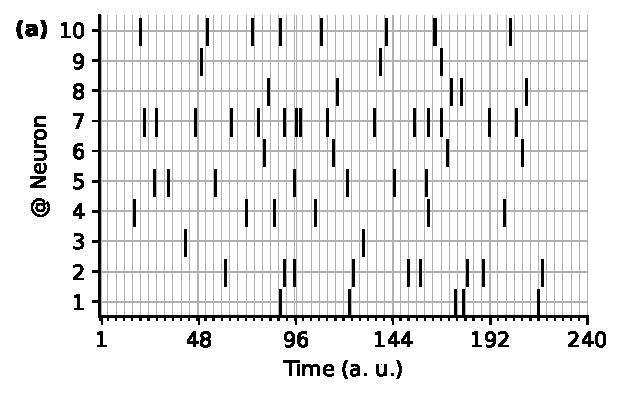
\includegraphics[width=.50\linewidth]{figures/THC_toy-a_k.pdf}
  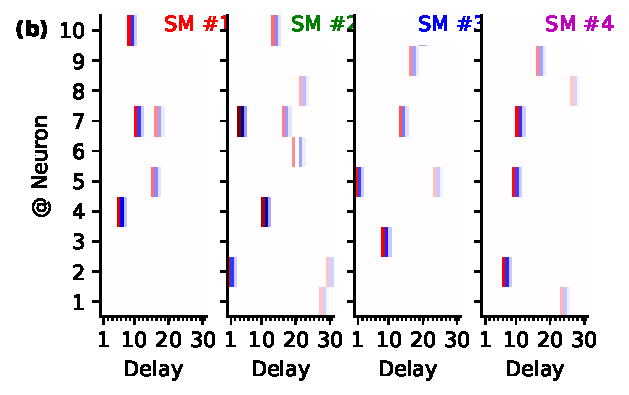
\includegraphics[width=.50\linewidth]{figures/THC_toy-b.pdf}\\
  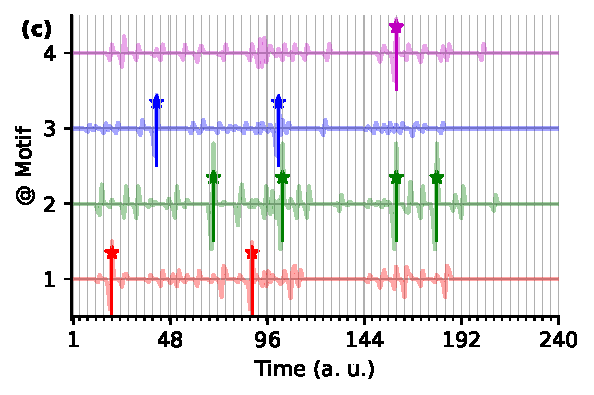
\includegraphics[width=.50\linewidth]{figures/THC_toy-c.pdf}
  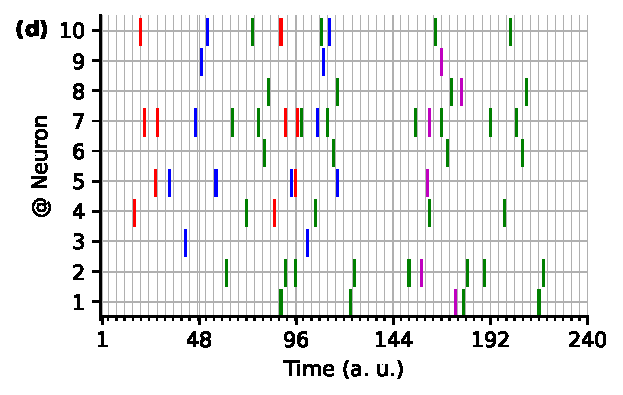
\includegraphics[width=.50\linewidth]{figures/THC_toy-a.pdf} 

\caption{Generating raster plots and inferring spiking motifs. \textbf{(a)}~As an illustration for the generative model, we draw a multiunit raster plot synthesized from $4$ different spiking motifs and for $10$ presynaptic neurons. \textbf{(b)}~We show these motifs, each identified at the top by a different color. The evidence of activation (red) or deactivation (blue) is assigned to each presynaptic neuron and $31$ different possible delays. \textbf{(c)}~The activation in time of the different motifs (denoted by stars) is drawn at random and then used to generate a raster plot on the multi-unit address space (see panel a). By inverting this model, an inference model can be defined for their efficient detection, outputting an evidence value (continuous line) from which the identity and timing of SMs can be inferred (vertical bars). \textbf{(d)}~The original raster plot can be annotated with each identified spiking motif.
}
\label{fig:THC}
\end{figure}
%---------------------------
\subsection{A generative model for raster plots}

As described in Figure~\ref{fig:izhikevich}, a spiking motif can be detected using a properly tuned HD-SNN that maximizes spike synchronization at the postsynaptic terminal. Taking the argument the other way around, one may form a generative model for realistic raster plots in which spikes in the presynaptic address space are generated as the conjunction of spiking motifs defined in the postsynaptic space, knowing that both populations are connected by a set of weights and delays whose structure is stable relatively to the coding timescale. When connection weights are strong and sparsely distributed, this firing will robustly cause a specific temporal motif. Overall, these examples show that raster plots may be considered as a mixture of the effects of different elementary causes, and that each event triggers a specific spatio-temporal spiking motif. 

Formally, the activation of spiking motifs can occur independently and at random times. The activity is represented as a boolean matrix $B\in \{0, 1\}^{M\times T}$, where $M$ is the number of different spiking motifs (see Figure~\ref{fig:THC}c). Each entry $B(\postsynaddr, t)$ indicates whether a particular motif $\postsynaddr$ is activated at time $t$. The firing of a neuron $\presynaddr$ at time $t$ is considered a Bernoulli trial with a bias parameter $p(\presynaddr, t) \in [0, 1]$. This bias is conditioned by the presence of spiking motifs on postsynaptic neurons with corresponding delays.
%Formally, spiking motifs may be activated independently and at random times, such that we write this activity as $B(\postsynaddr, t)=1$ if $b$ is activated at $t$ and else $B(\postsynaddr, t)=0$. This defines $B\in \{0, 1\}^{M\times T}$ as the raster plot corresponding to the temporal activation of the spiking motifs, where $M$ is the number of different spiking motifs (see Figure~\ref{fig:THC}c). The probability of firing of a neuron $a$ at a given time $t$ can be understood as a Bernoulli trial whose (only) parameter is a bias $p(\presynaddr, t) \in [0, 1]$. 
Assuming that this bias is conditioned by the presence of spiking motifs on \emph{all} efferent postsynaptic neurons with the corresponding delays, it can be shown that the logit (inverse of the sigmoid) of this probability bias can be written as the sum of the logit of each of these factors, whose values we will define as the corresponding weights in the kernel. We can thus write the probability bias $p(a, t)$ as the accumulated evidence given these factors as 
\begin{equation*}
p(\presynaddr, t) = \sigma\big(\kernel_\presynaddrspace(\presynaddr) + \sum_{\postsynaddr \in \synapse_\presynaddr, 0 \le \synapticdelay \le D} B(\postsynaddr, t+\synapticdelay) \cdot \kernel^\postsynaddr(\presynaddr, \synapticdelay) \big)  
\end{equation*}
where $\sigma$ is the sigmoid function. We will further assume that kernel's weights are balanced (their mean is zero) and that $\kernel_\presynaddrspace$ is a bias such that $\forall \presynaddr, t$, $\sigma(\kernel_\presynaddrspace(\presynaddr))$ is the average background firing rate. 
%Conveniently, one can write this summation as a one-dimensional temporal convolution operator such that we may simply write
% \begin{equation*}
% p = \sigma(\kernel_\presynaddrspace + B \ast \kernel )
% \end{equation*}
% where  $p\in [ 0, 1]^{N\times T}$ and $B\in \{0, 1\}^{M\times T}$ is the raster plot corresponding to the temporal activation of the spiking motifs. 
Finally, we obtain the raster plot $A\in \{0, 1\}^{N\times T}$ by drawing spikes using independent Bernoulli trials based on the computed probability biases $A \sim \mathcal{B}(p)$. Note that, depending on the definition of kernels, the generative model can model a discretized Poisson process, generate rhythmic activity or more generally propagating waves. This formulation thus defines a simple generative model for raster plots as a combination of independent spiking motifs.  This generative model can be easily extented to include a refractory period  with a parameter r (r>=1).  Refractory period ensures that there is a minimum time gap between successive action potentials, preventing them from overlapping. This temporal separation allows for discrete and well-defined neural signals, enabling accurate information processing and mitigating signal interference. The refractory period contributes to energy efficiency in neural systems and plays a crucial role in temporal coding by creating distinct time windows between successive spikes. 

%
%\subsection{Detecting event-based motifs using spiking neurons with heterogeneous delays}

%
\subsection{Detecting spiking motifs}
%: Detection model

%
%By discretizing time (here with an arbitrary time unit $1~\ms$), we can also define the motifs as a matrix giving the weight with respect to the different delays $d \in [0, D]$ (where $D$ is the maximum delay) at different addresses $a \in [1, N]$ where $N$ is the number of neurons from the multiunit recording. When a given motif is activated, it will produce a discharge pattern corresponding to that specific set of delays and addresses. Let's define the probability of firing of a neuron $a$ at a given time $t$ as a Bernoulli trial whose (only) parameter is a bias $p(a, t) \in [0, 1]$. For any given probability $p$ it is convenient to define the corresponding \emph{evidence} which corresponds to the log odds $\log \frac{p}{1-p} = \sigma^{-1}(p)$, where $\sigma$ is the sigmoid function. Assuming that the presence of spiking motifs is binary, it is easy to show that the total evidence can be written as the sum of these evidences, whose values are given by the corresponding weights. Assuming that we know that there are $M$ such motifs, we define $b \in [1, M]$ the address of a motif and $\kernel_b$ the corresponding weight matrices. This allows us to derive a generative model for raster plots (see \fig{THC}). 
%
 %Spiking motifs may be activated independently at random times and we write that $B(b, t)=1$ if $b$ is activated at $t$ (and otherwise $B(b, t)=0$). We can thus write the probability bias as the joint probability given these factors as $p(a, t) = \sigma\big(\kernel_0 + \sum_{b, t} B(b, t) \cdot \kernel_b(a, t-d) \big)$. We will further assume that the weights are balanced (their mean is zero) and that $\kernel_0$ is a bias such that $p_0=\sigma(\kernel_0)$ is the average background firing rate. Conveniently, this summation can be written as a one-dimensional temporal convolution operator, so we can simply write $p = \sigma(\kernel_0 + B \ast W )$ where  $p\in [ 0, 1]^{N\times T}$ and $B\in \{0, 1\}^{M\times T}$ is the raster plot corresponding to the temporal activation of the spiking motifs. Finally, we obtain the raster plot $A\in \{0, 1\}^{N\times T}$ by drawing spikes using independent Bernoulli trials $A \sim \mathcal{B}(p)$. Note that, depending on the shape of the kernels, the generative model can model a Poisson process, generate rhythmic activity or more generally propagating waves. This formulation thus defines a simple generative model for raster plots as a combination of independent spiking motifs. 
%Using this dense representation, the counting defined above becomes:
%\begin{equation*}
%\mathcal{C}^\postsynaddr(a,t)
%= \sum_{\presynaddr, \synapticdelay_\ranksyn^\postsynaddr} \kernel^\postsynaddr(\presynaddr_\ranksyn^\postsynaddr, \synapticdelay_\ranksyn^\postsynaddr) \cdot A(\presynaddr, \timev-\synapticdelay_\ranksyn^\postsynaddr)
%\end{equation*}
%%
%This shows that $\mathcal{C}^\postsynaddr$ is a temporal convolution of the dense representation of the event stream with the dense kernels formed by the set of synapses:  $\mathcal{C}^\postsynaddr = \kernel^\postsynaddr \ast A$.
%This well-known computation defines a time-invariant, differentiable measure which is very efficiently implemented for GPUs and which we will use for learning the classification of different motifs in the event stream.
%%
%
%\note{formalize the following:}
%More generally, every cause may be considered as occurring independently and one might write the generative model for the generation of the presynaptic events as:
%
%
%Using this formalization, one might now deduce an optimal algorithm for the detection of such temporal motifs.
%
%
%By discretization of time (with here an arbitrary unitary time unit), we can also define the dendrite as a matrix giving the weight corresponding to the different delays $d \in [0, D]$ (where $D$ is the maximum delay) on different pre-synaptic addresses $a \in [1, N]$ defining the list of the $N$ dendrites. We will denote as $W(a, d)$ these weights.
%
%
%Following the observations of~\cite{izhikevich_polychronization_2006}, let us assume that such precise discharge motif defines a polychronous group (PG). Assuming that we know there exists $M$ such groups, we will define as $b \in [1, M]$ the address of a PG and as $\kernel_b$ the corresponding weight matrices. This allows then to derive a generative model for raster plots (\fig{model}-(b)).


% 
Assuming the spiking motifs (as defined by the kernel $\kernel$) are known, the generative model allows to determine an inference model for detecting sources $\hat{B}$ when observing a raster plot $A$. Indeed, by using this forward model, it is possible to estimate the likelihood $p(b, t)$ for the presence of a spiking motif of address $b$ and at time $t$ by using the transpose convolution operator. This consists in using the emitting field $\synapse_\presynaddr$ of presynaptic neurons in place of the receptive field $\synapse^\postsynaddr$ of postsynaptic neurons. It thus comes that when observing $A$, then one may infer the logit of the probability as the sum of evidences:
\begin{equation*}
  p(\postsynaddr, t) = \sigma\big(\kernel_\postsynaddrspace(b) + \sum_{\presynaddr \in \synapse^\postsynaddr,  0 \le \synapticdelay \le D} A(\presynaddr, t-\synapticdelay) \cdot \kernel^T_\presynaddr(\postsynaddr, \synapticdelay) \big)  
\end{equation*}
This also takes the form of a temporal convolution. This assumption holds as long as the kernels are uncorrelated, a condition which is met here numerically by choosing a relatively sparse set of synapses (approximately $1\%$ of active synapses). Finally, we compute $\hat{B}$ by selecting the most likely items, allowing to identify the spiking motifs in the input raster plot (see Figure~\ref{fig:THC}d). 

One may naturally extend this algorithm when the spiking motifs (that is, the weights) are not known, but that we know the timing and identity of the spiking motifs. Indeed, the equation above is differentiable. Indeed, the activation function of our spiking neural is a sigmoid function implementing a form of  Multinomial Logistic Regression (MLR)~\cite{grimaldi_learning_2023}.  
The underlying metric is the binary cross-entropy, as used in the logistic regression model. In particular, if we consider kernels with similar decreasing exponential time profile, one can prove that this detection model is similar to the method of~\cite{berens_fast_2012}. In our specific case, the difference is that the regression is performed in both dendritic and delay space by extending the summation using a temporal convolution operator. 

%\subsection{Implementation using spiking neurons with heterogeneous delays}
%
% The activation function of our spiking neural is a softmax function implementing a form of  Multinomial Logistic Regression (MLR)~\cite{grimaldi_robust_2023}, in analogy to a spiking Winner-Take-All network~\cite{nessler_bayesian_2013}. 
%It transforms this list of weights into a probability with the following formula:
%$
%Pr(k=\postsynaddr \; \vert \; \timev) =
%\frac 1 Z
%{\exp  (\mathcal{C}^\postsynaddr(\timev) +\bias^\postsynaddr) }
%$ 
%where $\mathcal{C}^\postsynaddr(\timev) = \sum
%\activeweights^\postsynaddr(t)
%$ is the sum of the synaptic weights and $\bias^\postsynaddr$ is the bias linked to neuron $\postsynaddr$. 
%In particular, we expect that some specific motifs may become tightly synchronized as they reach the basal dendritic tree, leading to a high postsynaptic activity which makes it progressively more likely to generate an output spike.
%%
%
% \note{say that it is effortless in biology but difficult on conventional computers}
% In our MLR model with $\Nclass=\Nspeed$ classes, a probability value is predicted for each event at address $\presynaddr_\arank$ and at time $\timev_\arank$ as a softmax function of the linear combination of the list of events on the basal dendrite of a neuron $\postsynaddr$ in association to a specific class. The linear combination can be defined by a set of synapses $\synapse^\postsynaddr$ as described in the heterogeneous delays model. 
%
\section{Results}
%
To quantify the efficiency of this operation, we generated $M=144$ synthetic spiking motifs as random independent kernels over $N=128$ presynaptic inputs and $D=31$ possible delays. We drew random independent instances of $B$ with a length of $T=1000$ time steps and an average of $1.0$ spikes per neuron. This allowed us to generate raster plots, which we use to infer $\hat{B}$. We compute accuracy as the rate of true positive detections (both for inferring the address and its exact timing) and observe on average $\approx 98\%$ correct detections.

We extended this result by showing how accuracy evolves as a function of the number of simultaneous spiking motifs, holding the frequency of occurrence constant. We show in \fig{model_results}~(left) that the accuracy of finding the right spiking motif is still above $80\%$ accuracy with more than $1364$ overlapping spiking motifs. This observation illustrates quantitatively the capacity  of the HD-SNN in representing a high number of simultaneous patterns. Furthermore, we show in \fig{model_results}~(middle) that (with $M=144$ spiking motifs fixed) the accuracy increases significantly with increasing temporal depth $D$ of the spiking motif kernel, quantitatively demonstrating the computational advantage of using heterogeneous delays. These results were obtained under the assumption that we know the $\kernel$. However, this is generally not the case, for example, when considering the raster plot of a population of neurons.

Finally, we evaluated the performance of the supervised learning scheme in inferring the connection kernel when the address and timing of spiking motifs are known. The kernel was initialized with random independent values, and we used stochastic gradient descent with a learning rate of \num{1e-4} over $\num{1e4}$ trials (i.e., over rasters as defined above with $T=1000$ and $N=128$). Qualitatively, the convergence was monotonous, and the correct values of the $M=144$ spike motifs were quickly recovered. Quantitatively, the correlation between the true and learned kernel weights showed that all kernels were correctly recovered (see Figure~\ref{fig:model_results}, right). Performing inference with the learned weights was as efficient as with the true kernels, and showed no significant difference (not shown).

% In the following, we will define a generic visual task and determine a learning algorithm to solve that challenging task. %Inspired by the k-means algorithm, it is possible to devise a self-supervised learning algorithm. Our preliminary results show that it is possible to retrieve spiking motifs embedded in the data, yet that further analysis is necessary to improve the convergence of the algorithm. In particular, it seems promising to use a sparseness constraint in the inference mechanism such as to remove spurious correlations in the inference.

%---------------------------
\begin{figure}%[t!]
  \centering
  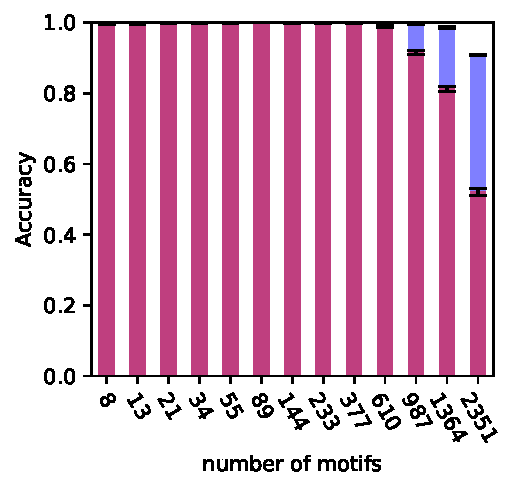
\includegraphics[width=0.335\linewidth]{figures/THC_N_SMs.pdf}
%  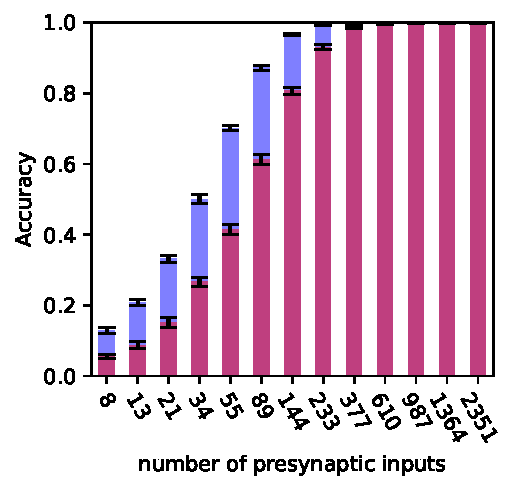
\includegraphics[width=0.320\linewidth]{figures/THC_N_pre.pdf}
  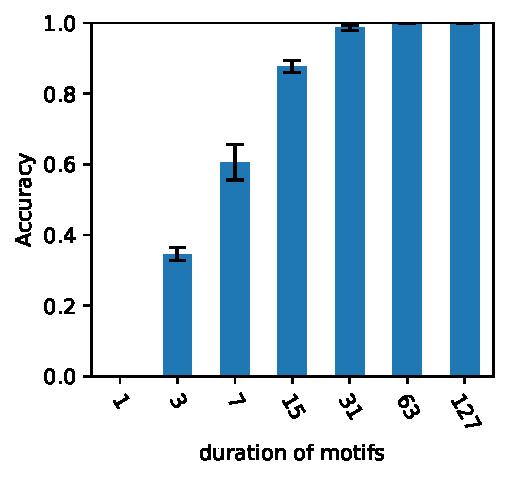
\includegraphics[width=0.330\linewidth]{figures/THC_N_SM_time.pdf} 
  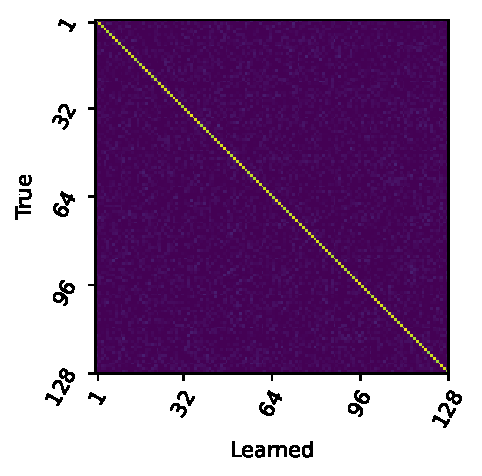
\includegraphics[width=0.315\linewidth]{figures/THC_xcorr-supervised.pdf}
    \caption{Detecting spiking motifs using spiking neurons with heterogeneous delays. 
Accuracy of detection for the classical correlation (red) and the HD-SNN method (blue) as a function of  {\bf (Left)}~the number $M$ of kernels, 
    %{\bf (Middle)}~the number of presynaptic neurons, 
    {\bf (Middle)}~the temporal depth $D$ of kernels among $M=144$ kernels.
    {\bf (Right)} Correlation matrix of true vs learned kernels.
    }
  \label{fig:model_results}
\end{figure}
%---------------------------
%
\section{Discussion}
%
\subsection{Synthesis and Main Contributions}
%%%-----------------------------------------------------------------
In summary, in this paper we have introduced a heterogeneous delay SNN model that we have evaluated for the detection of spiking motifs in a synthetic model of neurobiologically-inspired raster plots. 

We highlight some innovations in the contributions of this paper. First, the generic heterogeneous model is formalized from first principles for optimal detection of event-based spatiotemporal motifs. The model is evaluated on realistic data, while models like the tempotron are tested on simplified problems~\cite{gutig_tempotron_2006}. We have shown that the model accurately detects the exact identity and timing of spiking motifs, even when many are superimposed, provided that the spiking motifs are known. Compared to methods that use a correlation-based heuristic~\cite{ghosh_spatiotemporal_2019,yu_stsc-snn_2022}, our method is found to be more efficient. 

Second, compared to other event-based methods such as HOTS~\cite{lagorce_hots_2017}, the weights are explainable. They are directly related to the logit (inverse sigmoid of the probability) of detecting each spatiotemporal spike motif. Finally, another novelty is that while, for example, the polychronization model~\cite{izhikevich_polychronization_2006} learns only the weights using STDP, this model learns the weights and the delays simultaneously.%

\subsection{Main limits}
%%%----------------------------------------------------------------- %We have tested the effect of the size of the time bin and shown that it has essentially no effect on the results presented in this paper. This is consistent with the relative robustness of other event-based frameworks such as HOTS~\cite{lagorce_hots_2017}, where accuracy was unaffected when the input spikes were subjected to noisy perturbations up to $1~\ms$~\cite{grimaldi_robust_2023}. 
We have identified several limitations of the model, which we will now discuss. First, the entire framework is based on discrete time binning. This is incompatible with the continuous nature of biological time. We took advantage of this binning to efficiently implement the framework on conventional hardware, particularly GPUs, and in particular to leverage one-dimensional temporal convolutions.
However, it is possible to extend the HD-SNN formalism to a purely event-based SNN framework~\cite{grimaldi_robust_2023} by analytically including a precision term in the temporal value of the input spikes. As a result, promising speedups and energy gains for such computations could be achieved with such a purely event-based scheme.

Another limitation is that this model is purely feed-forward. Thus, the spikes produced by the postsynaptic neurons are generated solely on the basis of information contained in the classical receptive field. However, it is well known that neurons in the same layer can interact via lateral interactions, for example in V1, and that this can be the basis for computational principles~\cite{chavane_revisiting_2022}. Furthermore, neural information is modulated by feedback information, e.g. to distinguish a figure from its background~\cite{roelfsema_early_2016}, and it has been shown that feedback may be essential for building realistic models of primary visual areas~\cite{boutin_sparse_2020}, especially to explain non-linear mechanisms~\cite{boutin_effect_2020}. It is currently not possible to implement these recurrent connections in our implementation (lateral or feedback), mainly due to our use of convolutions. However, the generic theoretical model is able to incorporate them by inserting new spikes into the list of spikes reaching presynaptic addresses. While theoretically possible, in practice this must be properly tuned so that these recurrent connections do not amplify neuronal activity out of homeostatic state (by extinction or explosion).

For the implementation of predictive or anticipatory processes, such recurrent activity would be essential. This is essential in a neural system because it contains multiple different delays that require temporal alignment~\cite{hogendoorn_predictive_2019}. This has already been modeled to explain the flash-lag illusion~\cite{khoei_flash-lag_2017}. As noted above, this could be implemented using generalized coordinates (i.e., variables such as position supplemented by velocity, acceleration, jerk, \ldots), and ``neurobiologically, using delay operators just means changing synaptic connection strengths to take different mixtures of generalized sensations and their prediction errors''~\cite{perrinet_active_2014}. Our proposed heterogeneous delay model provides an alternative and elegant implementation solution to this problem.
%
\subsection{Perspectives}
%%%-----------------------------------------------------------------
% learning
The coding results were obtained under the assumption that we know the kernel $\kernel$, or using supervised learning by knowing the identity and timing of spiking motifs. However, this is generally not the case, e.g. when observing the neurobiological raster plot of a population of neurons. One perspective would be to extend the model to a fully self-supervised learning paradigm, i.e. without any labeled data~\cite{barlow_unsupervised_1989}. This type of learning is thought to be prevalent in the central nervous system and, assuming the signal is sparse~\cite{olshausen_emergence_1996}, one could extend these Hebbian sparse learning schemes to spikes~\cite{perrinet_emergence_2004,masquelier_competitive_2009}. 

We expect that this would be particularly useful for exploring neurobiological data~\cite{mackevicius_unsupervised_2019}. Indeed, there is a large literature showing that brain dynamics often organize into stereotyped sequences such as synfire chains~\cite{ikegaya_synfire_2004}, packets~\cite{luczak_sequential_2007}, or hippocampal sequences~\cite{pastalkova_internally_2008,villette_internally_2015} (for a review, see~\cite{grimaldi_precise_2023}). These motifs are stereotyped and robust, as they can be activated in the same motif from day to day~\cite{haimerl_internal_2019}. In contrast to conventional methods used to process neurobiological data, such an event-based model would be able to answer key questions regarding the representation of information in neurobiological data. Furthermore, it would open possibilities in the field of machine learning, especially in computer vision, to address current key concerns such as robustness to attacks, scalability, interpretability, or energy consumption.

Inspired by the k-means algorithm, it is possible to develop a self-supervised learning algorithm for the automatic detection of spiking motifs. For this, we can initialize $\kernel$ at random and define an auto-encoder scheme that infers the sources $\hat{B}$ for each input $A$ and then resynthesizes the corresponding raster plot. A natural metric is again binary cross-entropy, as used in the logistic regression model. Since the model is differentiable, we can optimize $\kernel$ using gradient descent. We can add a homeostatic regularization on the average firing rate of $B$ to ensure that each motif was \emph{a priori} equally activated~\cite{perrinet_adaptive_2019}. Our preliminary results show that it is possible to retrieve spiking motifs embedded in synthetic data. However, further analysis is needed to improve the convergence of the algorithm and to apply such algorithms to real neurobiological data. In particular, it seems promising to use a sparseness constraint in the inference mechanism to remove spurious correlations in the inference.
%
\bibliographystyle{splncs04}
%
\bibliography{polychronies}
%
% \begin{thebibliography}{10}
%   \providecommand{\url}[1]{\texttt{#1}}
%   \providecommand{\urlprefix}{URL }
%   \providecommand{\doi}[1]{https://doi.org/#1}
  
%   % \bibitem{aronov_non-euclidean_2004}
%   % Aronov, D., Victor, J.D.: Non-{Euclidean} properties of spike train metric spaces. Physical Review E  \textbf{69}(6),  061905 (Jun 2004). \doi{10.1103/PhysRevE.69.061905}
  
%   \bibitem{barlow_unsupervised_1989}
%   Barlow, H.: Unsupervised {Learning}. Neural Computation  \textbf{1}(3),  295--311 (Sep 1989). \doi{10.1162/neco.1989.1.3.295}
  
%   \bibitem{berens_fast_2012}
%   Berens, P., Ecker, A.S., Cotton, R.J., Ma, W.J., Bethge, M., Tolias, A.S.: A {Fast} and {Simple} {Population} {Code} for {Orientation} in {Primate} {V1}. Journal of Neuroscience  \textbf{32}(31),  10618--10626 (Aug 2012). \doi{10/f365rn}
  
%   % \bibitem{boutin_pooling_2022}
%   % Boutin, V., Franciosini, A., Chavane, F., Perrinet, L.U.: Pooling strategies in {V1} can account for the functional and structural diversity across species. PLOS Computational Biology  \textbf{18}(7),  e1010270 (2022). \doi{10.1371/journal.pcbi.1010270}
  
%   \bibitem{boutin_sparse_2020}
%   Boutin, V., Franciosini, A., Chavane, F.Y., Ruffier, F., Perrinet, L.U.: Sparse {Deep} {Predictive} {Coding} captures contour integration capabilities of the early visual system. PLoS Computational Biology  (May 2020). \doi{10.1371/journal.pcbi.1008629}
  
%   \bibitem{boutin_effect_2020}
%   Boutin, V., Franciosini, A., Ruffier, F., Perrinet, L.U.: Effect of top-down connections in {Hierarchical} {Sparse} {Coding}. Neural Computation  \textbf{32}(11),  2279--2309 (Feb 2020). \doi{10.1162/neco_a_01325}
  
%   \bibitem{chavane_revisiting_2022}
%   Chavane, F., Perrinet, L.U., Rankin, J.: Revisiting horizontal connectivity rules in {V1}: from like-to-like towards like-to-all. Brain Structure and Function  (Feb 2022). \doi{10.1007/s00429-022-02455-4}

%   \bibitem{ghosh_spatiotemporal_2019}
%   Ghosh, R., Gupta, A., Tang, S., Soares, A., Thakor, N.: Spatiotemporal {Feature} {Learning} for {Event}-{Based} {Vision}. arXiv:1903.06923 [cs]  (Mar 2019)

%   \bibitem{goodman_spike-timing-based_2010}
% Goodman, D.F.M., Brette, R.: Spike-timing-based computation in sound localization. PLoS Comput Biol  \textbf{6}(11) (Nov 2010). \doi{10.1371/journal.pcbi.1000993}, \url{http://www.ncbi.nlm.nih.gov/pmc/articles/PMC2978676/}

%   \bibitem{grimaldi_robust_2022}
%   Grimaldi, A., Boutin, V., Ieng, S.H., Benosman, R., Perrinet, L.: A robust event-driven approach to always-on object recognition  (Jan 2022). \doi{10/gn62xd}
  
%   \bibitem{grimaldi_precise_2022}
%   Grimaldi, A., Gruel, A., Besnainou, C., Martinet, J., Perrinet, L.U.: Precise {Spiking} {Motifs} in {Neurobiological} and {Neuromorphic} {Dat}. Tech. rep. (2022). \doi{10.3390/brainsci13010068}
  
%   \bibitem{grun_unitary_2002-1}
%   Grün, S., Diesmann, M., Aertsen, A.: Unitary events in multiple single-neuron spiking activity: {I}. {Detection} and significance. Neural Computation  \textbf{14}(1),  43--80 (Jan 2002). \doi{10.1162/089976602753284455}%, tex.ids= Grun2002
  
%   % \bibitem{grun_unitary_2010}
%   % Grün, S., Diesmann, M., Aertsen, A.: Unitary {Event} {Analysis}. In: Grün, S., Rotter, S. (eds.) Analysis of {Parallel} {Spike} {Trains}, pp. 191--220. Springer US, Boston, MA (2010). \doi{10.1007/978-1-4419-5675-0_10}
  
%   \bibitem{gutig_tempotron_2006}
%   Gütig, R., Sompolinsky, H.: The tempotron: a neuron that learns spike timing–based decisions. Nature Neuroscience  \textbf{9}(3),  420--428 (Mar 2006). \doi{10/ch29r4}
  
%   \bibitem{haimerl_internal_2019}
%   Haimerl, C., Angulo-Garcia, D., Villette, V., Reichinnek, S., Torcini, A., Cossart, R., Malvache, A.: Internal representation of hippocampal neuronal population spans a time-distance continuum. Proceedings of the National Academy of Sciences  \textbf{116}(15),  7477--7482 (Apr 2019). \doi{10/ghpbm3}
  
%   % \bibitem{hanuschkin_general_2010}
%   % Hanuschkin, A., Kunkel, S., Helias, M., Morrison, A., Diesmann, M.: A {General} and {Efficient} {Method} for {Incorporating} {Precise} {Spike} {Times} in {Globally} {Time}-{Driven} {Simulations}. Frontiers in Neuroinformatics  \textbf{4}, ~113 (Oct 2010). \doi{10.3389/fninf.2010.00113}
  
%   \bibitem{hogendoorn_predictive_2019}
%   Hogendoorn, H., Burkitt, A.N.: Predictive {Coding} with {Neural} {Transmission} {Delays}: {A} {Real}-{Time} {Temporal} {Alignment} {Hypothesis}. eneuro  \textbf{6}(2),  ENEURO.0412--18.2019 (Mar 2019). \doi{10/ggcrbj}
  
%   \bibitem{ikegaya_synfire_2004}
%   Ikegaya, Y., Aaron, G., Cossart, R., Aronov, D., Lampl, I., Ferster, D., Yuste, R.: Synfire {Chains} and {Cortical} {Songs}: {Temporal} {Modules} of {Cortical} {Activity}. Science  \textbf{304}(5670),  559--564 (Apr 2004). \doi{10/djckcn}
  
%   \bibitem{izhikevich_polychronization_2006}
%   Izhikevich, E.M.: Polychronization: {Computation} with spikes. Neural Computation  \textbf{18}(2),  245--282 (Feb 2006). \doi{10.1162/089976606775093882}%, \url{https://doi.org/10.1162/089976606775093882}, publisher: MIT Press One Rogers Street, Cambridge, MA 02142-1209, USA journals-info … tex.ids= izhikevich2006polychronization
  
%   \bibitem{khoei_flash-lag_2017}
%   Khoei, M.A., Masson, G.S., Perrinet, L.U.: The {Flash}-{Lag} {Effect} as a {Motion}-{Based} {Predictive} {Shift}. PLOS Computational Biology  \textbf{13}(1),  e1005068 (Jan 2017). \doi{10.1371/journal.pcbi.1005068}%, \url{https://journals.plos.org/ploscompbiol/article?id=10.1371/journal.pcbi.1005068}, tex.ids= Khoei2017a publisher: Public Library of Science
  
%   \bibitem{kreuz_measuring_2007}
%   Kreuz, T., Haas, J.S., Morelli, A., Abarbanel, H.D.I., Politi, A.: Measuring spike train synchrony. Journal of Neuroscience Methods  \textbf{165}(1),  151--161 (Sep 2007). \doi{10.1016/j.jneumeth.2007.05.031}
  
%   \bibitem{lagorce_hots_2017}
%   Lagorce, X., Orchard, G., Galluppi, F., Shi, B.E., Benosman, R.B.: {HOTS}: {A} {Hierarchy} of {Event}-{Based} {Time}-{Surfaces} for {Pattern} {Recognition}. IEEE Transactions on Pattern Analysis and Machine Intelligence  \textbf{39}(7),  1346--1359 (2017). \doi{10.1109/TPAMI.2016.2574707}%, \url{http://www.ncbi.nlm.nih.gov/pubmed/27411216%20http://ieeexplore.ieee.org/document/7508476/}, tex.ids= Lagorce2017a tex.bdsk-url-2: https://doi.org/10.1109/TPAMI.2016.2574707 tex.date-added: 2020-11-09 16:16:25 +0100 tex.date-modified: 2020-11-09 16:16:25 +0100 url: http://www.ncbi.nlm.nih.gov/pubmed/27411216 http://ieeexplore.ieee.org/document/7508476/ 
  
%   \bibitem{levakova_review_2015}
%   Levakova, M., Tamborrino, M., Ditlevsen, S., Lansky, P.: A review of the methods for neuronal response latency estimation. Biosystems  \textbf{136},  23--34 (Oct 2015). \doi{10.1016/j.biosystems.2015.04.008}%, \url{https://doi.org/gpshjz}, this CSL Item was generated by Manubot v0.5.2 from its persistent identifier (standard\_id). standard\_id: doi:10.1016/j.biosystems.2015.04.008
  
%   \bibitem{luczak_sequential_2007}
%   Luczak, A., Barthó, P., Marguet, S.L., Buzsáki, G., Harris, K.D.: Sequential structure of neocortical spontaneous activity in vivo. Proceedings of the National Academy of Sciences  \textbf{104}(1),  347--352 (Jan 2007). \doi{10.1073/pnas.0605643104}%, \url{https://www.pnas.org/content/104/1/347}, tex.ids= Luczak2007a publisher: National Academy of Sciences section: Biological Sciences
  
%   \bibitem{mackevicius_unsupervised_2019}
%   Mackevicius, E.L., Bahle, A.H., Williams, A.H., Gu, S., Denisenko, N.I., Goldman, M.S., Fee, M.S.: Unsupervised discovery of temporal sequences in high-dimensional datasets, with applications to neuroscience. eLife  \textbf{8},  e38471 (Feb 2019). \doi{10.7554/eLife.38471}%, \url{https://doi.org/10.7554/eLife.38471}, publisher: eLife Sciences Publications, Ltd
  
%   \bibitem{masquelier_competitive_2009}
%   Masquelier, T., Guyonneau, R., Thorpe, S.J.: Competitive {STDP}-{Based} {Spike} {Pattern} {Learning}. Neural Computation  \textbf{21}(5),  1259--1276 (May 2009). \doi{10/dds34f}%, \url{http://www.mitpressjournals.org/doi/10.1162/neco.2008.06-08-804}, 00203
  
%   \bibitem{olshausen_emergence_1996}
%   Olshausen, B.A., Field, D.J.: Emergence of simple-cell receptive field properties by learning a sparse code for natural images. Nature  \textbf{381}(6583),  607--609 (1996). \doi{10/dvj4qz}%, \url{http://dx.doi.org/10.1038/381607a0 http://www.ncbi.nlm.nih.gov/htbin-post/Entrez/query?db=m&form=6&dopt=r&uid=8637596 http://www.ncbi.nlm.nih.gov/pubmed/8637596 http://www.nature.com/doifinder/10.1038/381607a0}, 00000
  
%   \bibitem{pachitariu_robustness_2018}
%   Pachitariu, M., Stringer, C., Harris, K.D.: Robustness of {Spike} {Deconvolution} for {Neuronal} {Calcium} {Imaging}. The Journal of Neuroscience  \textbf{38}(37),  7976--7985 (2018). \doi{10.1523/jneurosci.3339-17.2018}%, \url{https://doi.org/gd9mcx}, this CSL Item was generated by Manubot v0.5.2 from its persistent identifier (standard\_id). standard\_id: doi:10.1523/jneurosci.3339-17.2018
  
%   \bibitem{pastalkova_internally_2008}
%   Pastalkova, E., Itskov, V., Amarasingham, A., Buzsáki, G.: Internally {Generated} {Cell} {Assembly} {Sequences} in the {Rat} {Hippocampus}. Science (New York, N.Y.)  \textbf{321}(5894),  1322--1327 (Sep 2008). \doi{10.1126/science.1159775}%, \url{https://www.ncbi.nlm.nih.gov/pmc/articles/PMC2570043/}, tex.ids= Pastalkova2008a
  
%   \bibitem{perrinet_emergence_2004}
%   Perrinet, L.: Emergence of filters from natural scenes in a sparse spike coding scheme. Neurocomputing  \textbf{58-60}(C),  821--826 (2004). \doi{10.1016/j.neucom.2004.01.133}%, \url{http://linkinghub.elsevier.com/retrieve/pii/S0925231204001389}, tex.ids: Perrinet03 tex.date-modified: 2019-02-22 11:55:28 +0100
  
%   % \bibitem{perrinet_role_2010}
%   % Perrinet, L.U.: Role of homeostasis in learning sparse representations. Neural computation  \textbf{22}(7),  1812--36 (2010). \doi{10.1162/neco.2010.05-08-795}%, \url{http://www.mitpressjournals.org/doi/10.1162/neco.2010.05-08-795 http://www.ncbi.nlm.nih.gov/pubmed/20235818 http://www.pubmedcentral.nih.gov/articlerender.fcgi?artid=PMC2929690 http://arxiv.org/abs/0706.3177 http://www.incm.cnrs-mrs.fr/LaurentPerrinet/Pub}, tex.ids= Perrinet10, Perrinet10shl, Perrinet2010a tex.bdsk-url-2: https://doi.org/10.1162/neco.2010.05-08-795 tex.date-modified: 2019-09-02 15:45:35 +0200 tex.eprint: 20235818 tex.eprinttype: pmid tex.preprint: https://hal-amu.archives-ouvertes.fr/hal-00156610 tex.publisher: MIT Press tex.url: https://arxiv.org/abs/0706.3177 tex.url\_code: https://laurentperrinet.github.io/publication/perrinet-10-shl publisher: MIT Press url: https://arxiv.org/abs/0706.3177
  
%   \bibitem{perrinet_adaptive_2019}
%   Perrinet, L.U.: An adaptive homeostatic algorithm for the unsupervised learning of visual features. Vision  \textbf{3}(3), ~47 (2019). \doi{10/ggkdks}%, \url{https://github.com/SpikeAI/HULK}, 00000 tex.date-added: 2019-09-01 16:14:10 +0300 tex.date-modified: 2019-09-19 12:00:01 +0200 tex.grants: anr-horizontal-v1,spikeai; mesocentre tex.preprint: https://laurentperrinet.github.io/publication/perrinet-19-hulk/ tex.time\_start: 2019-04-18T13:00:00 tex.url: https://spikeai.github.io/HULK/ tex.url\_code: https://github.com/SpikeAI/HULK
  
%   \bibitem{perrinet_active_2014}
%   Perrinet, L.U., Adams, R.A., Friston, K.J.: Active inference, eye movements and oculomotor delays. Biological Cybernetics  \textbf{108}(6),  777--801 (Dec 2014). \doi{10/f6skjq}%, \url{https://doi.org/10.1007/s00422-014-0620-8}, tex.ids= Perrinet14a, Perrinet2014a, Perrinet2014b tex.date-modified: 2020-03-31 11:07:29 +0200 tex.eprint: 25128318 tex.eprinttype: pmid tex.preprint: https://hal-amu.archives-ouvertes.fr/hal-01382350 publicationTitle: Biological cybernetics publisher: Springer Berlin Heidelberg url: http://link.springer.com/article/10.1007\%2Fs00422-014-0620-8
  
%   % \bibitem{perrinet_edge_2015}
%   % Perrinet, L.U., Bednar, J.A.: Edge co-occurrences can account for rapid categorization of natural versus animal images. Scientific reports  \textbf{5},  11400 (2015). \doi{10.1038/srep11400}%, tex.ids= Perrinet2015, Perrinet2015d, PerrinetBednar15 tex.bdsk-url-2: https://doi.org/10.1038/srep11400 tex.date-added: 2020-03-27 10:11:37 +0100 tex.date-modified: 2020-03-27 10:11:44 +0100 tex.grants: anr-bala-v1 tex.preprint: https://hal-amu.archives-ouvertes.fr/hal-01202447 tex.url\_code: https://github.com/laurentperrinet/PerrinetBednar15 publisher: Nature Publishing Group url: http://dx.doi.org/10.1038/srep11400
  
%   \bibitem{riehle_spike_1997}
%   Riehle, A., Grun, S., Diesmann, M., Aertsen, A.: Spike synchronization and rate modulation differentially involved in motor cortical function. Science (New York, N.Y.)  \textbf{278}(5345),  1950--1953 (1997). \doi{10.1126/science.278.5345.1950}%, tex.ids= Riehle1997a publisher: American Association for the Advancement of Science
  
%   \bibitem{roelfsema_early_2016}
%   Roelfsema, P.R., de~Lange, F.P.: Early visual cortex as a multiscale cognitive blackboard. Annual review of vision science  \textbf{2},  131--151 (2016). \doi{10.1146/annurev-vision-111815-114443}%, publisher: Annual Reviews
  
%   \bibitem{van_rossum_novel_2001}
%   van Rossum, M.C.: A novel spike distance. Neural Computation  \textbf{13}(4),  751--763 (Apr 2001). \doi{10.1162/089976601300014321}
  
%   \bibitem{stella_comparing_2022}
%   Stella, A., Bouss, P., Palm, G., Grün, S.: Comparing {Surrogates} to {Evaluate} {Precisely} {Timed} {Higher}-{Order} {Spike} {Correlations}. eneuro  \textbf{9}(3),  ENEURO.0505--21.2022 (2022). \doi{10.1523/eneuro.0505-21.2022}%, \url{https://doi.org/gqjvht}, this CSL Item was generated by Manubot v0.5.2 from its persistent identifier (standard\_id). standard\_id: doi:10.1523/eneuro.0505-21.2022
  
%   \bibitem{victor_nature_1996}
%   Victor, J.D., Purpura, K.P.: Nature and precision of temporal coding in visual cortex: a metric-space analysis. Journal of Neurophysiology  \textbf{76}(2),  1310--1326 (Aug 1996). \doi{10.1152/jn.1996.76.2.1310}%, \url{https://www.physiology.org/doi/10.1152/jn.1996.76.2.1310}
  
%   \bibitem{villette_internally_2015}
%   Villette, V., Malvache, A., Tressard, T., Dupuy, N., Cossart, R.: Internally {Recurring} {Hippocampal} {Sequences} as a {Population} {Template} of {Spatiotemporal} {Information}. Neuron  \textbf{88}(2),  357--366 (Oct 2015). \doi{10/f7whnn}%, \url{https://www.sciencedirect.com/science/article/pii/S0896627315008417}, 00085
  
%   \bibitem{williams_point_2020}
%   Williams, A.H., Degleris, A., Wang, Y., Linderman, S.W.: Point process models for sequence detection in high-dimensional neural spike trains. Tech. rep. (Oct 2020)%, \url{http://arxiv.org/abs/2010.04875}, 00003 tex.ids= Williams2020a arXiv: 2010.04875 rights: http://creativecommons.org/licenses/by/4.0/
  
%   \bibitem{yu_stsc-snn_2022}
%   Yu, C., Gu, Z., Li, D., Wang, G., Wang, A., Li, E.: {STSC}-{SNN}: {Spatio}-{Temporal} {Synaptic} {Connection} with {Temporal} {Convolution} and {Attention} for {Spiking} {Neural} {Networks} (Oct 2022)%, \url{http://arxiv.org/abs/2210.05241}, arXiv:2210.05241 [cs, q-bio, stat]
  
%   \end{thebibliography}
  
\end{document}
 